\newpage

\section*{Extended Data}

\renewcommand{\figurename}{Extended Data Fig.}
\renewcommand{\tablename}{Extended Data Table}
% \renewcommand{\thetable}{S\arabic{table}}
% \algrenewcommand\algorithmicrequire{\textbf{Model parameter:}}
\begin{algorithm}
\caption{Generative model for pixel intensities}
\label{alg:pseudocode}
\begin{algorithmic}[1]
\Require $\gamma$ (floated)
\Comment{camera gain}
\Require $\pi^z$ (floated)
\Comment{average on-target spot probability}
\Require $\pi^j$ (floated)
\Comment{average off-target spot probability}
\Require $\sigma^{xy} = 0.5 $ (fixed)
\Comment{std of on-target spot position (pixels)}
\Require $\nu^{xy} = \left( \dfrac{P+1}{2 \sigma^{xy}} \right)^2 - 1 $
\Comment{reparameterization of $\sigma^{xy}$}
\Require $\sigma^{h} = 10000$ (fixed)
\Comment{scale of intensity distribution (a.u.)}
\Require $\{\mu^b_n\}^N_{n=1}, \{\sigma^b_n\}^N_{n=1}$ (floated)
\Comment{mean and std of background intensity (a.u.)}
\Require $w_{\min} = 0.75, w_{\max} = 2.25$ (fixed)
\Comment{width range (pixels)}
\Require $\{ \delta_r \}^R_{r=1}, \bm{\pi}^\delta$ (fixed)
\Comment{empirical offset samples and weights}
\ForAll{target sites $n \in \{1 \dots N\}$}
    \ForAll{frames $f \in \{1 \dots F\}$}
    \Comment{time-independent}
        \State $b_{nf} \sim \textbf{Gamma}(\mu^b_n, \sigma^b_n)$
        \Comment{draw background intensity}
        \State $\theta_{nf} \sim \textbf{Categorical}_{1,\dots,K}(\dfrac{1}{K}, \dots, \dfrac{1}{K})$
        \Comment{draw on-target spot index}
        
        \ForAll{spots $k \in \{1 \dots K\}$}
            \State $ m_{knf} \sim
                    \begin{cases}
                    \textbf{Bernoulli}(\pi^z) & \text{$\theta_{nf} = k$ (on-target)} \\
                    \textbf{Bernoulli}(\pi^j) & \text{$\theta_{nf} \neq k$ (off-target)}
                    \end{cases} $
            \Comment{draw spot presence indicator}
            \If{$m_{knf}=1$}
            \Comment{if spot is present}
                \State $h_{knf} \sim \textbf{HalfNormal}(\sigma^h)$
                \Comment{draw spot intensity}
                \State $w_{knf} \sim \textbf{Uniform}(w_{\min}, w_{\max})$
                \Comment{draw spot width}
                \State $ x_{knf} \sim
                        \begin{cases}
                        \textbf{AffineBeta}(0, \nu^{xy}, -\frac{P+1}{2}, \frac{P+1}{2}) & \text{$\theta_{nf} = k$} \\
                        \textbf{Uniform}(-\frac{P+1}{2}, \frac{P+1}{2}) & \text{$\theta_{nf} \neq k$}
                        \end{cases}$
                \Comment{draw $x$-axis center}
                \State $ y_{knf} \sim
                        \begin{cases}
                        \textbf{AffineBeta}(0, \nu^{xy}, -\frac{P+1}{2}, \frac{P+1}{2}) & \text{$\theta_{nf} = k$ (on-target)} \\
                        \textbf{Uniform}(-\frac{P+1}{2}, \frac{P+1}{2}) & \text{$\theta_{nf} \neq k$ (off-target)}
                        \end{cases}$
                \Comment{draw $y$-axis center}
            \EndIf
        \EndFor
            
        \ForAll{pixels $i,j \in \{1 \dots P\}$}
            \ForAll{spots $k \in \{1 \dots K\}$}
                \State $\mu^{S}_{knfij} =
                        \begin{cases}
                            \dfrac{h_{knf}}{2 \pi w^2_{nfk}} \exp{\left ( -\dfrac{(i-x_{nfk})^2 + (j-y_{nfk})^2}{2w^2_{nfk}} \right)} & \text{if $m_{knf} = 1$} \\
                            0 & \text{otherwise}
                        \end{cases}$
                \Comment{2D Gaussian spot}
            \EndFor
            \State $\mu^I_{nfij} = b_{nf} + \sum_k \mu^S_{knfij}$
            \Comment{mean pixel intensity w/o offset}
            \State $I_{nfij} \sim \textbf{Gamma} (\mu^I_{nfij}, \sqrt{\mu^I_{nfij} \gamma})$
            \Comment{draw pixel intensity w/o offset}
            \State $\delta_{nfij} \sim \textbf{Categorical}_{\{ \delta_r \}^R_{r=1}}(\bm{\pi}^\delta)$
            \Comment{draw offset signal}
            \State \Return $D_{nfij} = \delta_{nfij} + I_{nfij}$
            \Comment{observed pixel intensity}
        \EndFor
    \EndFor
\EndFor
\end{algorithmic}
\end{algorithm}

\setcounter{figure}{0}

\begin{figure}[t]
\centering
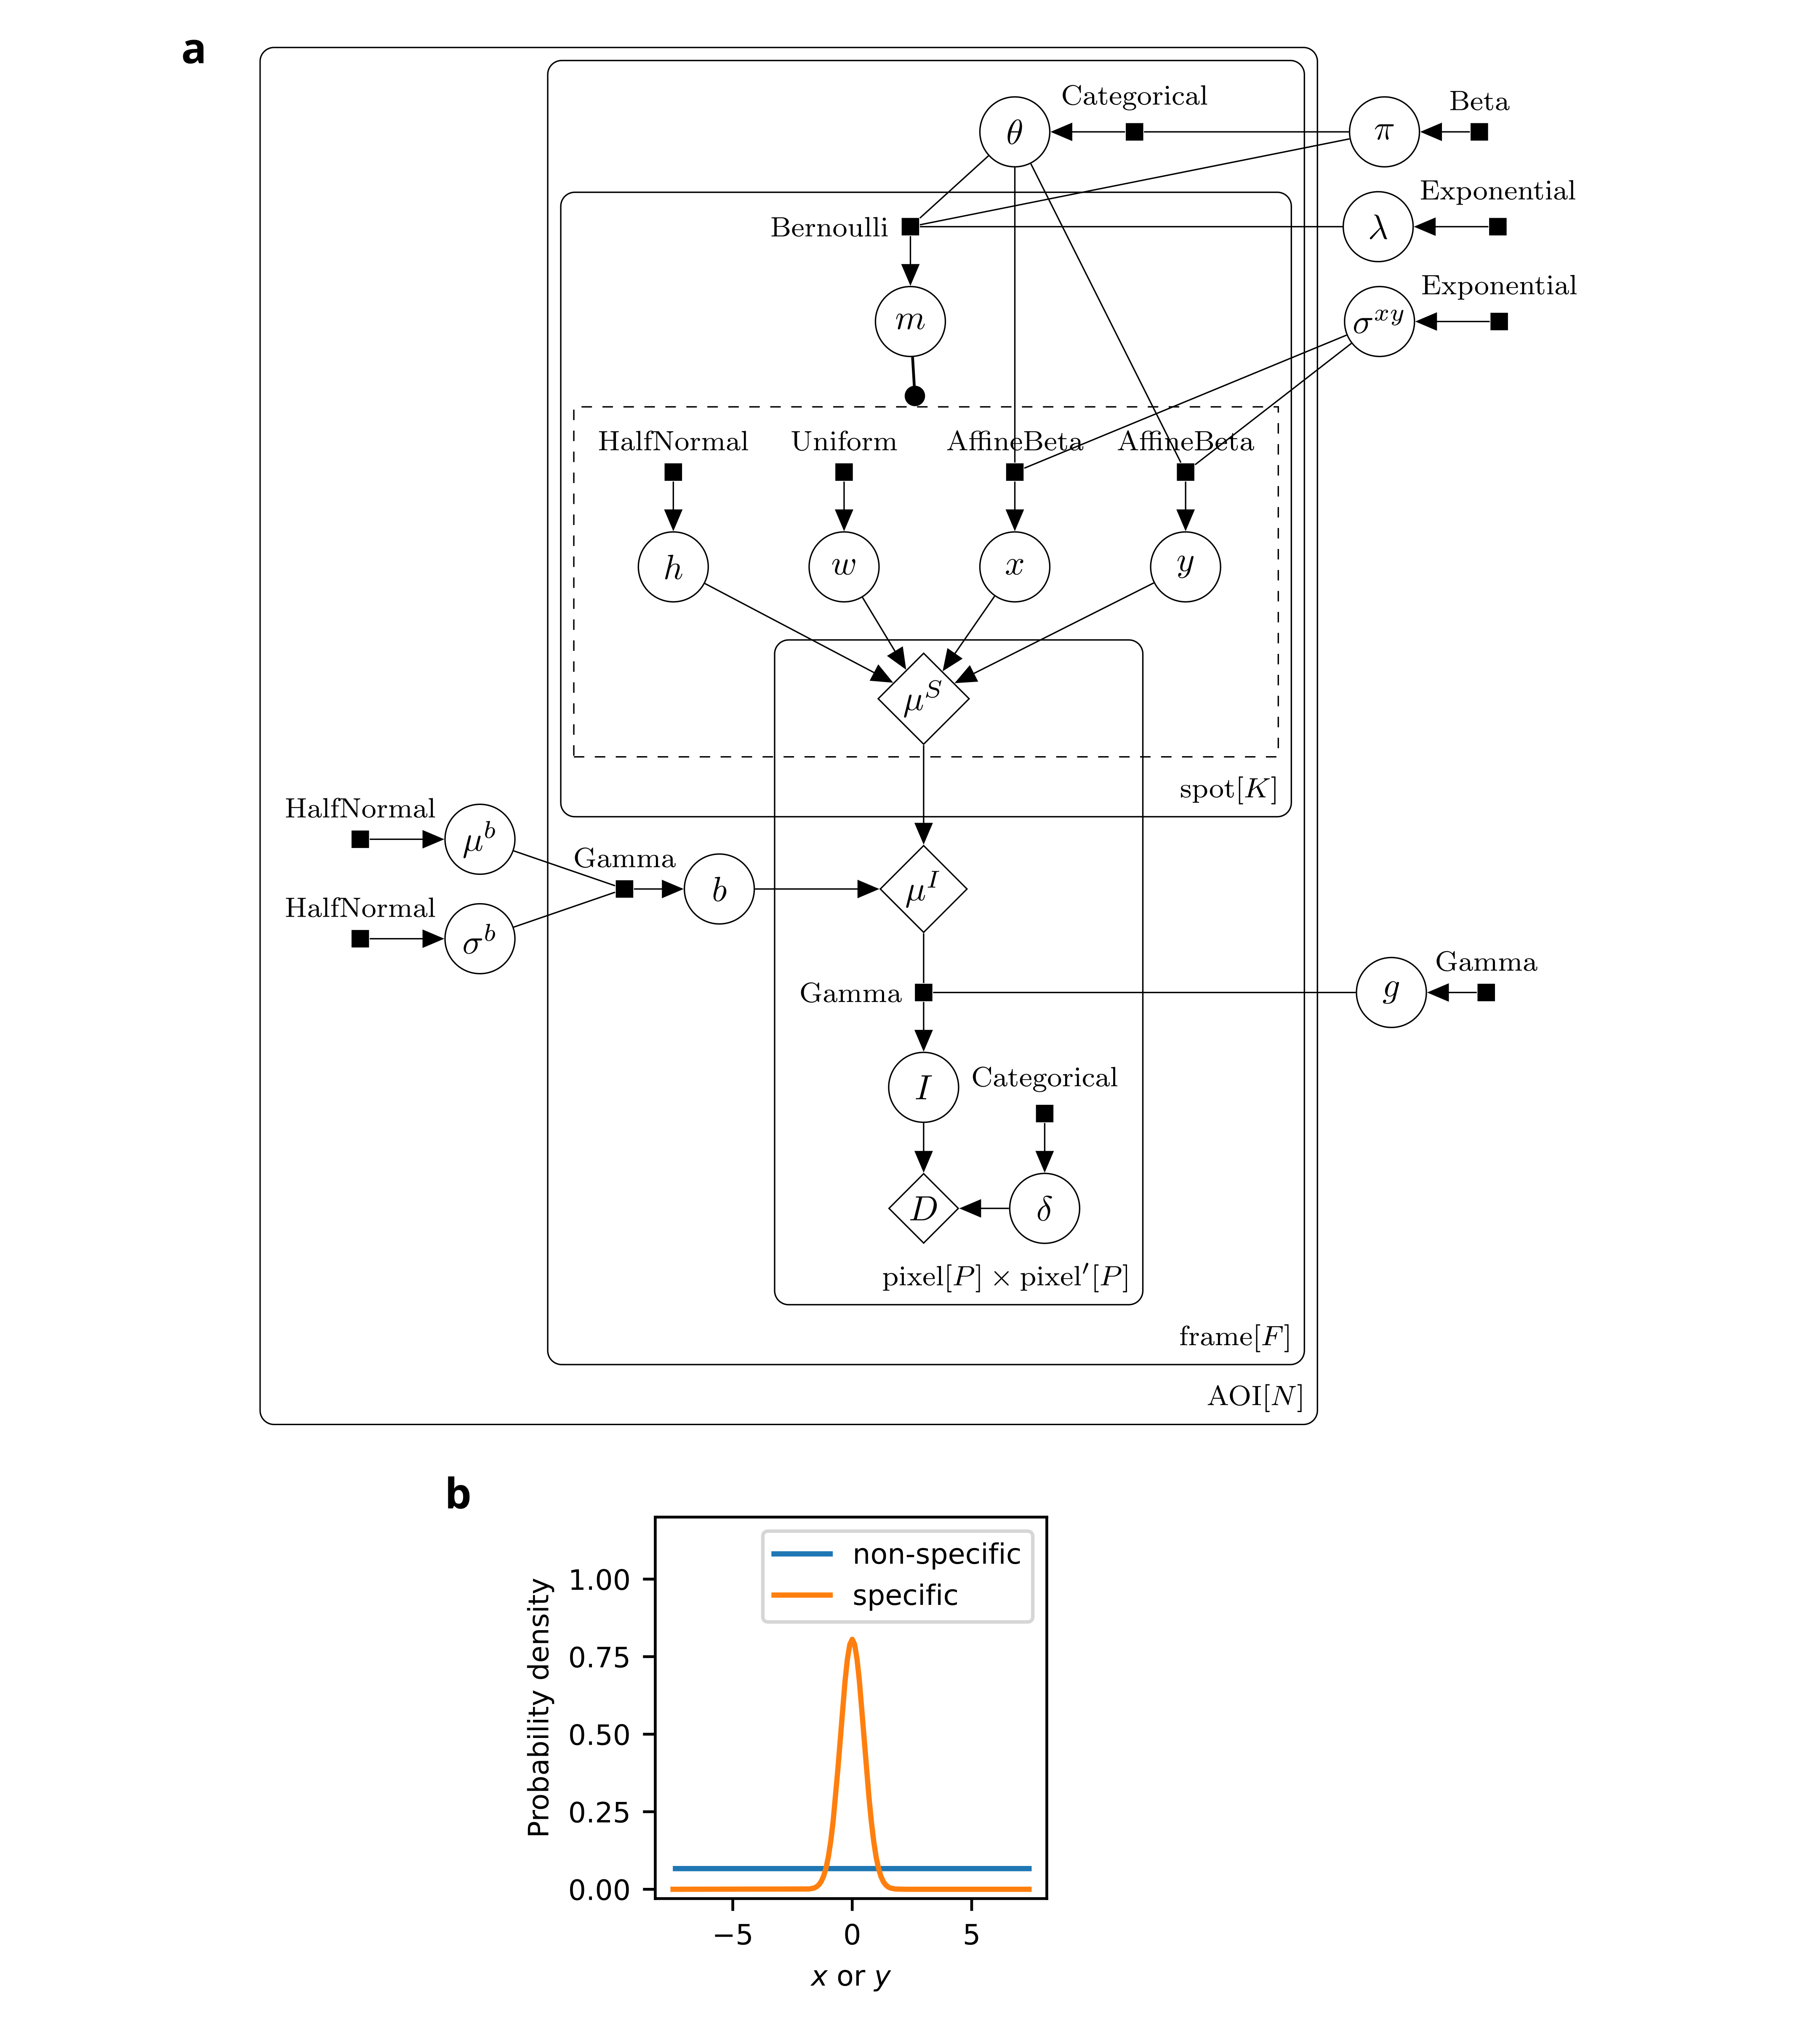
\includegraphics[width=183mm]{figures/sup1/sup1.png}
\label{fig:full_model}
\end{figure}

%\addtocounter{figure}{-1}
\begin{figure} [t!]
\caption{\textbf{Extended graphical representation of the generative probabilistic model and the prior distributions for $x$ and $y$ spot position parameters.} \textbf{a}, Directed factor graph representation (ref) of model parameters and parameter distributions. Model parameters are depicted as circles, parameter distributions as small filled squares, and deterministic functions as diamonds. Names of the probability distributions are written next to the squares. Input parameters and output parameters are connected by lines, with an arrow pointing towards the dependent parameter. Observed image $D$ is the sum of the noisy photon-dependent image $I$ and the photon-independent camera offset $\delta$. The dashed box represents selection of spot parameters based on the spot existence indicator $m$. Plates (rounded rectangles) contain nodes that are repeated for the number of instances displayed at the bottom-right corner: number of AOIs ($N$), frame count ($F$), maximum number of spots in a single image ($K=2$), and number of image pixels ($P \times P$). \textbf{b}, Prior distributions of $x$ and $y$ for specific and non-specific binding. Probability densities for $x$ and $y$ are defined in the range of the image $-(P+1)/2$, $(P+1)/2$ and are conditional on the identity of the spot (specific or non-specific).  Probability densities for $x$ and $y$ parameters are identical. }
\end{figure}


\begin{figure}[t]
\centering
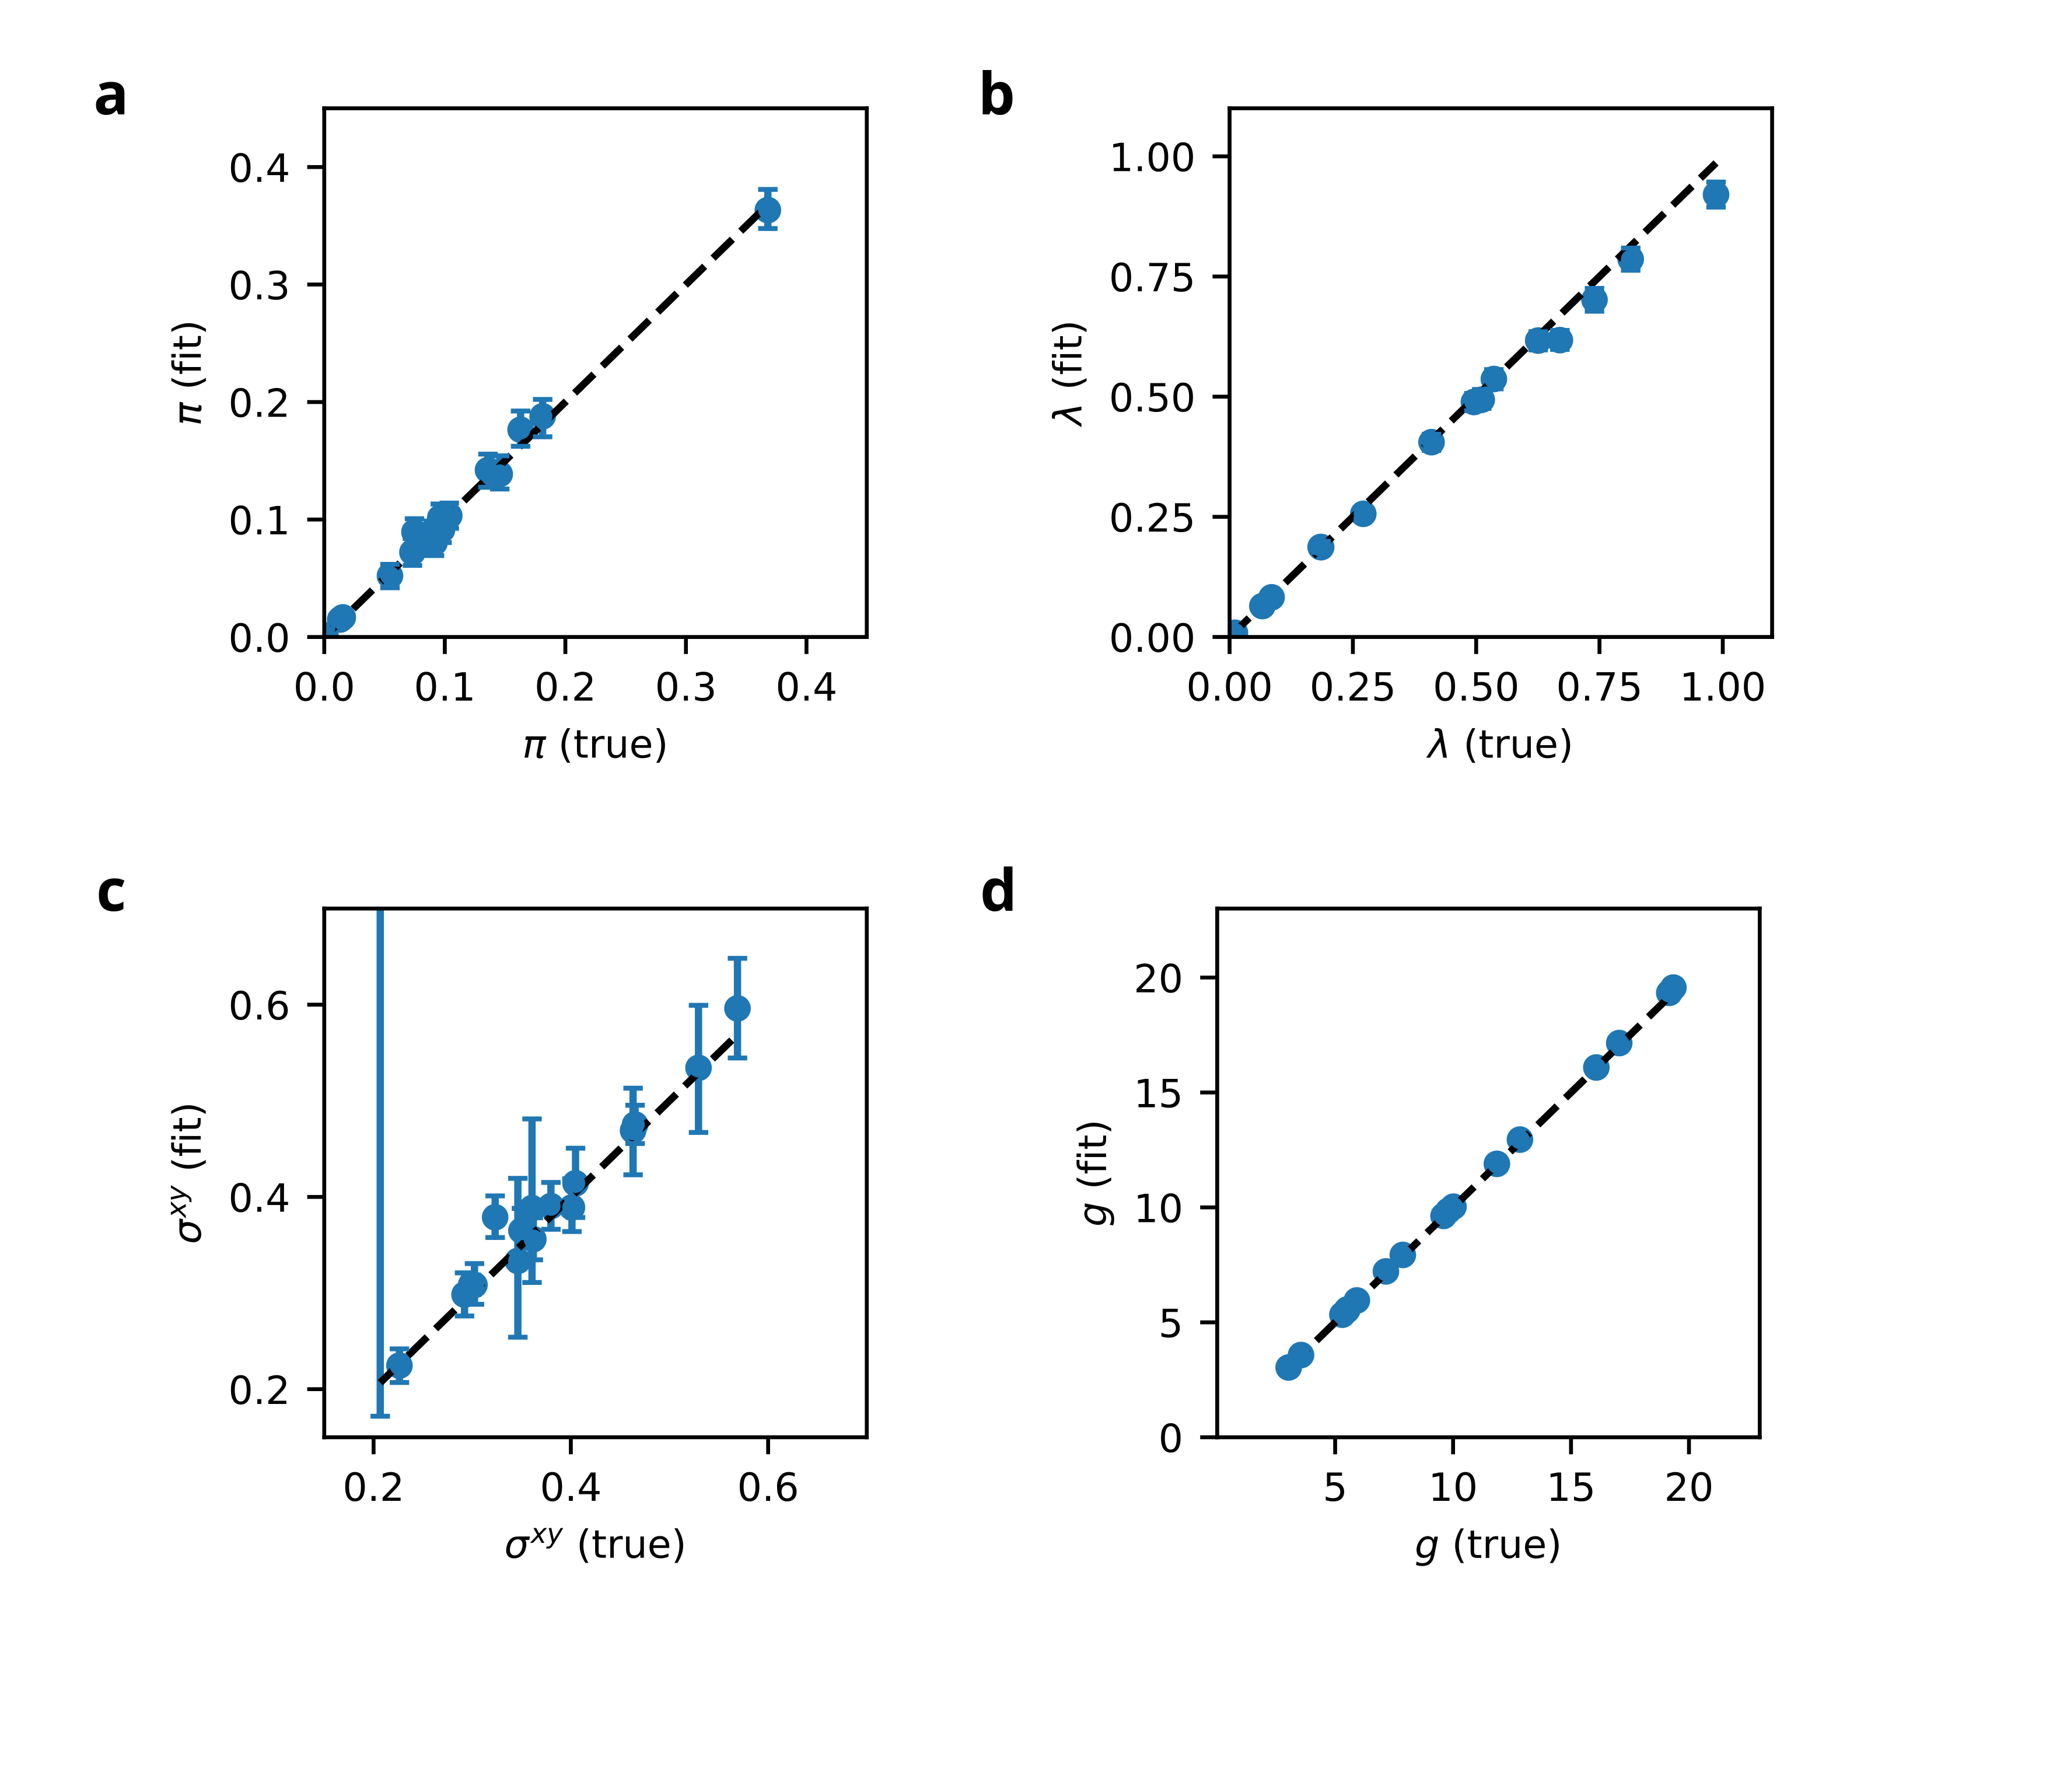
\includegraphics[width=150mm]{figures/sup2/sup2.png}
\caption{\textbf{Tapqir analysis of image data simulated using a broad range of global parameters.} Simulations (see Methods) consist of 16 datasets where global parameters ($\pi$, $\lambda$, $\sigma^{xy}$, and $g$) where randomly generated for each dataset. Simulated data were fit with Tapqir, and parameter values from the fit are plotted against the true parameter values (circles). To guide the eye, dashed lines  indicate identical true and fit values. \textbf{a}, Average specific binding probability $\pi$. \textbf{b}, Nonspecific binding rate $\lambda$. \textbf{c}, Proximity parameter $\sigma^{xy}$. \textbf{d}, Gain of the camera $g$. }
\label{fig:tapqir_global}
\end{figure}

\begin{figure}[t]
\centering
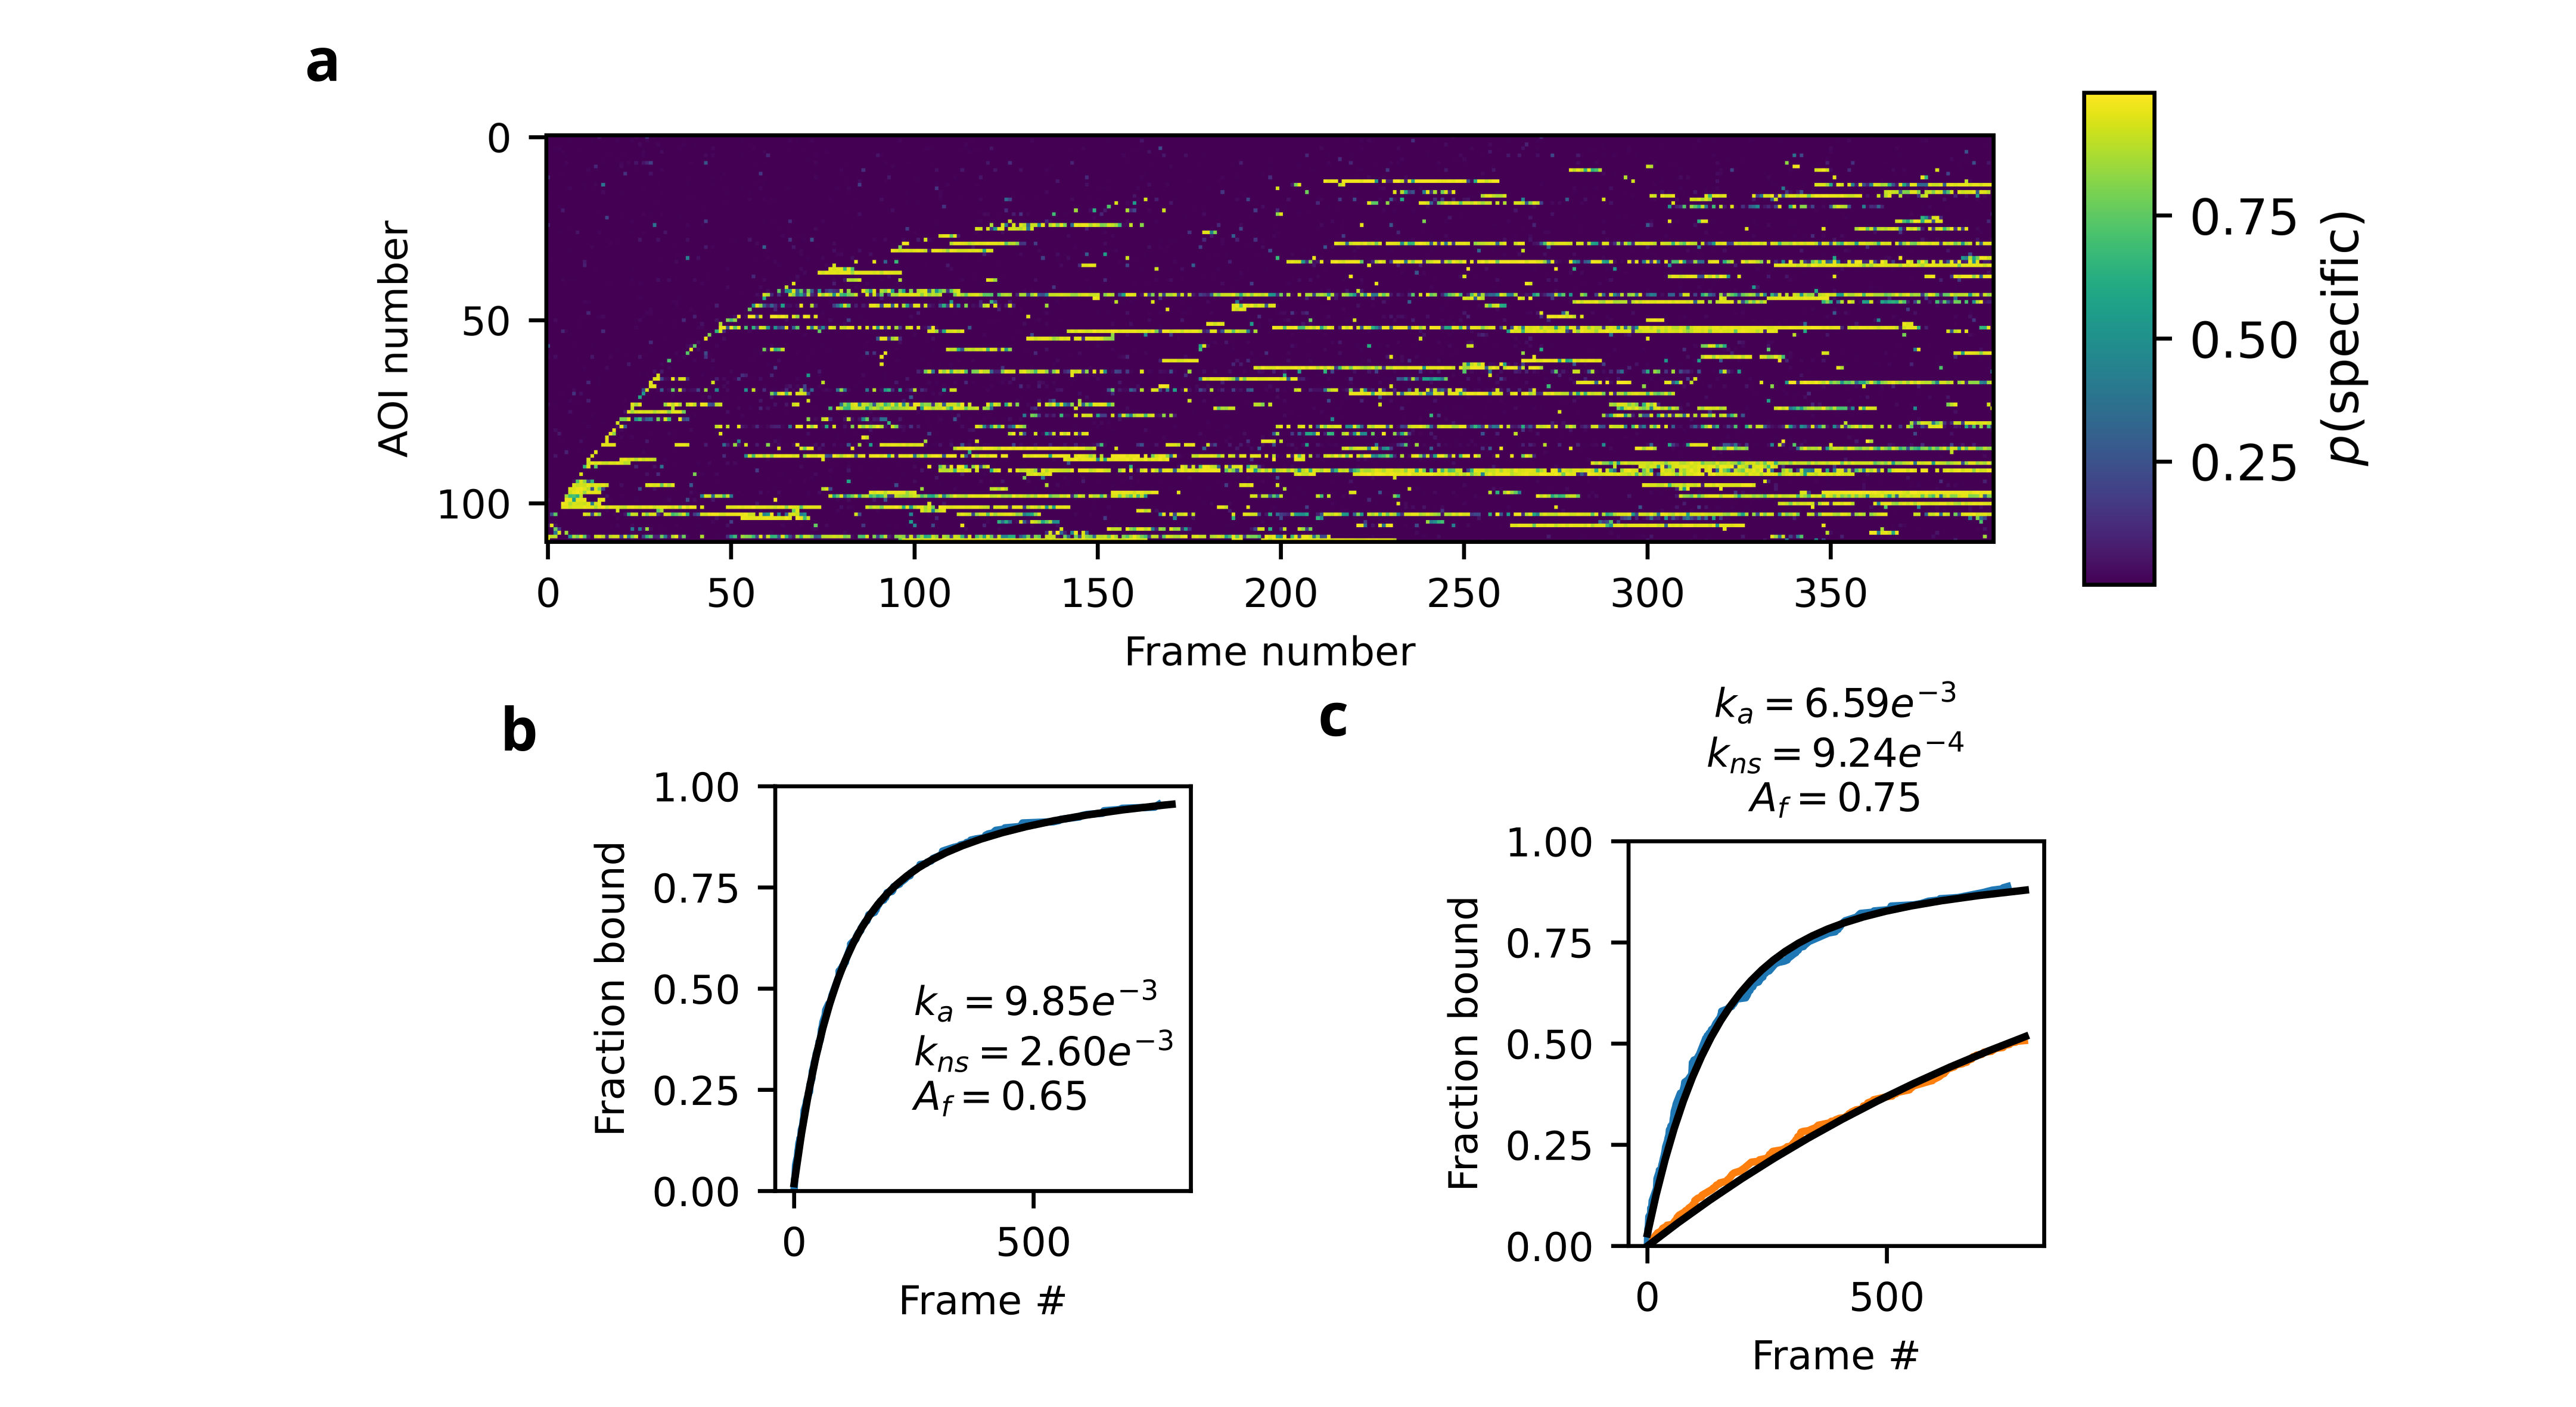
\includegraphics[width=183mm]{figures/sup3/sup3.png}
\caption{\textbf{Time-to-first binding analysis of experimental data.}  Determining association rates for experimental CoSMoS data using the time-to first binding analysis. \textbf{a}, Rastergrams of PolII target-specific presence probabilities $p(\mathsf{specific})$ (green scale) at DNA locations ordered by time-to-first binding. Data set: PolII in Table S1. \textbf{b}, Time-to first binding analysis of classification results from Tapqir. Fraction bound (blue) plotted as a function of time. Black line is simulated using best-fit values for $k_\mathrm{a}$, $k_\mathrm{ns}$, and $A_\mathrm{f}$. \textbf{c}, Same as in (b) but for spotpicker analysis. Orange is fraction bound for negative control data.
}
\label{fig:experimental_data}
\end{figure}

\begin{figure}[t]
\centering
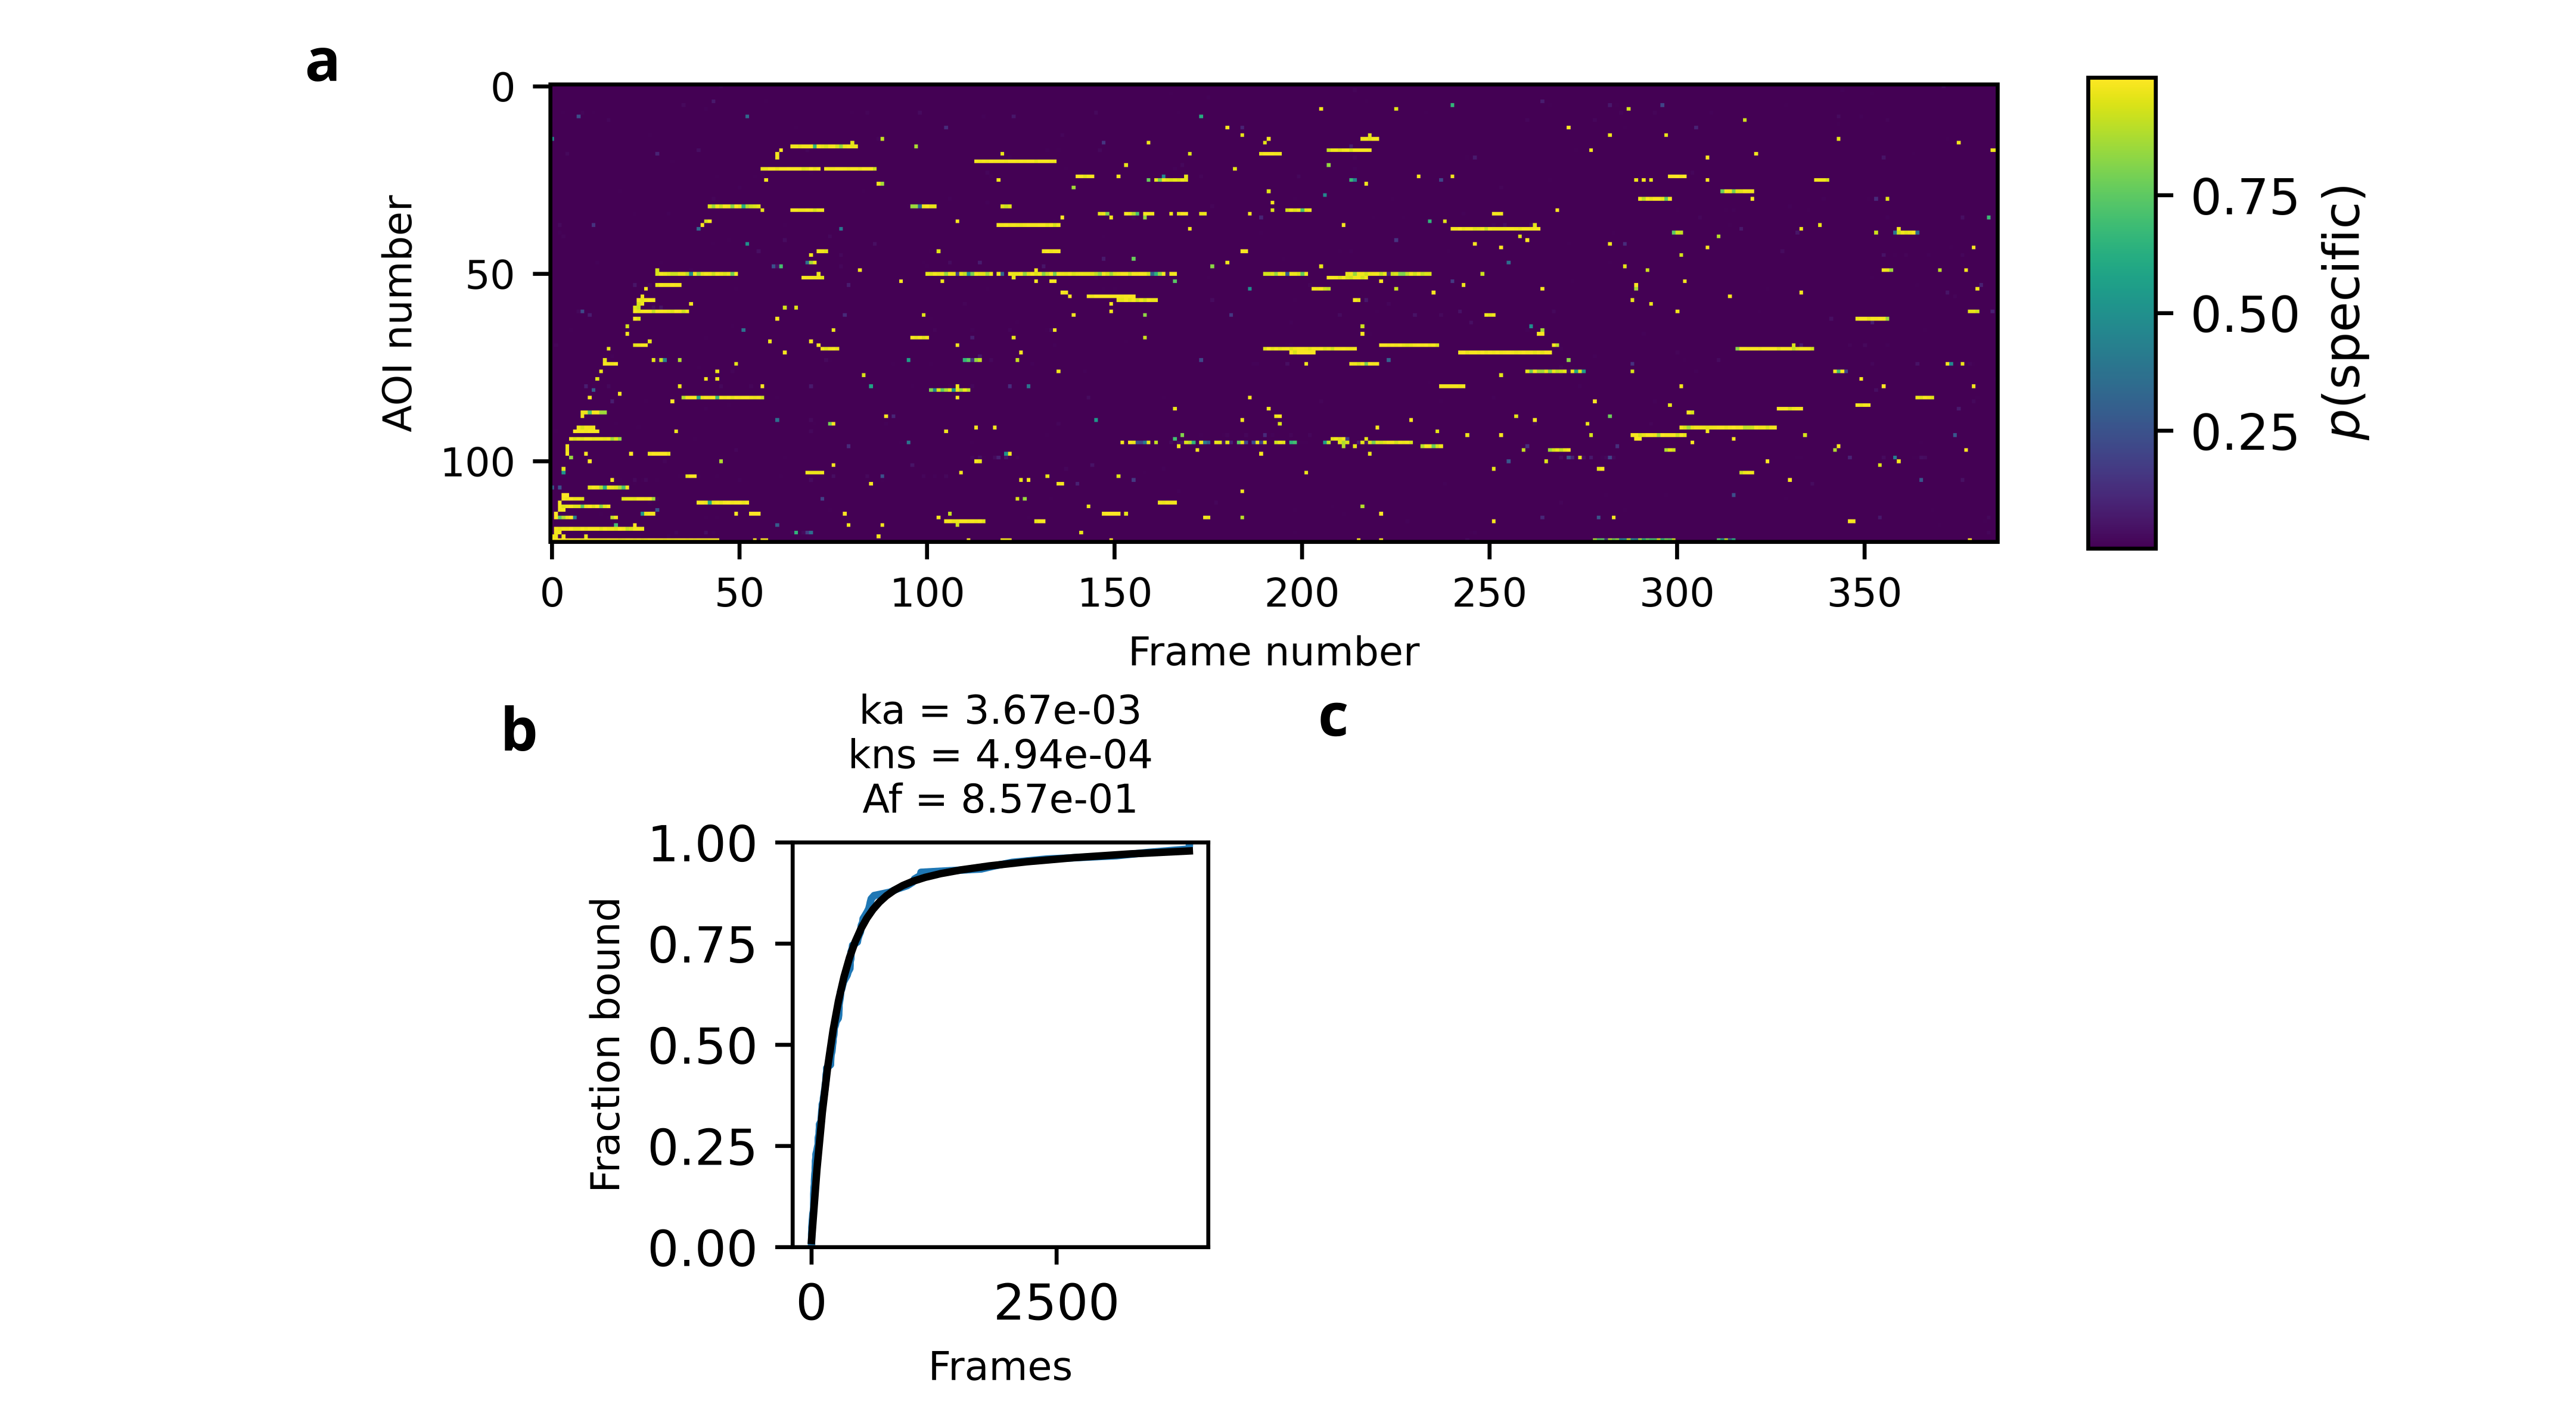
\includegraphics[width=183mm]{figures/sup4/sup4.png}
\caption{\textbf{Time-to-first binding analysis of experimental data.}  Determining association rates for experimental CoSMoS data using the time-to first binding analysis. \textbf{a}, Rastergrams of PolII target-specific presence probabilities $p(\mathsf{specific})$ (green scale) at DNA locations ordered by time-to-first binding. Data set: PolII in Table S1. \textbf{b}, Time-to first binding analysis of classification results from Tapqir. Fraction bound (blue) plotted as a function of time. Black line is simulated using best-fit values for $k_\mathrm{a}$, $k_\mathrm{ns}$, and $A_\mathrm{f}$. \textbf{c}, Same as in (b) but for spotpicker analysis. Orange is fraction bound for negative control data.
}
\label{fig:experimental_data}
\end{figure}

\begin{table}
\caption{\label{tab:example} \textbf{Experimental datasets.}}
% Use "S" column identifier to align on decimal point 
\begin{tabular}{lrrrrrr}
\toprule
Dataset & size & SNR & $\pi$ & $\lambda$ & $g$ & $\sigma^{xy}$ \\
\midrule
polII & \begin{tabular}[x]{@{}c@{}}$N = 331$, $F = 790$\\$N_c = 526$, $F_c = 526$\end{tabular} & 1.61 &
0.114 & 0.320 & 6.43 & 0.575 \\
\midrule
NusG & \begin{tabular}[x]{@{}c@{}}$N = 122$, $F = 3855$\\$N_c = 157$, $F_c = 3855$\end{tabular} & 4.37 & $0.030$ & $0.0772$ & $16.91$ & $0.384$ \\
\midrule
$\sigma^{54}$ & \begin{tabular}[x]{@{}c@{}}$N = 102$, $F = 4407$\\$N_c = 127$, $F_c = 4407$\end{tabular} & 3.87 & 0.073 & 0.149 & 11.414 & 0.448 \\
\bottomrule
\multicolumn{7}{l}{\footnotesize{\parbox{5in}{$^{1}$Data description}}} \\
\end{tabular}
\end{table}

$\sigma^{54}$ - Single molecule experiment measuring the binding rate of $\sigma^{54}$RNAP labeled with Cy3 to DNA where the target site for the polymerase on the DNA was bracketed different length (598P255) blue in Fig. 1E in https://www.pnas.org/content/pnas/110/24/9740.full.pdf.

$\sigma^{54}$ - 598P2993

\pagebreak

\newcommand{\specialcell}[2][c]{%
  \begin{tabular}[#1]{@{}r@{}}#2\end{tabular}}

\begin{table}
\caption{\label{tab:example} \textbf{Simulated datasets from randomized global parameters (Figure S2).}}
\begin{tabular}{lrrrrrr}
\toprule
Dataset &  $\textrm{SNR}^2$ &  $\pi$ &  $\lambda$ &  $g$ &  $\sigma^{xy}$ \\
\midrule
\specialcell{seed0\\\vphantom{fg}}  &  \specialcell{2.409\\2.443}  &   \specialcell{$1.46 \times 10^{-1}$\\$(1.25, 1.53) \times 10^{-1}$}  &  \specialcell{$5.11 \times 10^{-1}$\\$[0.474, 0.513]$} & \specialcell{$17.04$\\$[17.104, 17.198]$}  &  \specialcell{$0.362$\\$(0.332, 0.378)$} \\
\midrule
\specialcell{seed1\\\vphantom{fg}}  & \specialcell{5.276\\5.456} &       \specialcell{$1.36 \times 10^{-1}$\\$(1.28, 1.56) \times 10^{-1}$}  &  \specialcell{$4.95 \times 10^{-1}$\\ $0.51 \pm$}  &  \specialcell{$3.55$ \\ $17.68 \pm$}  &  \specialcell{$0.380$ \\ $(0.366, 0.414)$} \\
\midrule
\specialcell{seed2\\\vphantom{fg}}  & \specialcell{2.272\\2.319} &       \specialcell{$1.81 \times 10^{-1}$\\$(1.70, 2.03) \times 10^{-1}$}  &  \specialcell{$6.70 \times 10^{-1}$\\ $0.51 \pm$}  &  \specialcell{$1.92 \times 10^{1}$ \\ $17.68 \pm$}  &  \specialcell{$0.323$ \\ $(0.359, 0.398)$} \\
\midrule
\specialcell{seed3\\\vphantom{fg}}  & \specialcell{4.232\\4.381} &       \specialcell{$9.04 \times 10^{-2}$\\$(7.68, 9.89) \times 10^{-2}$}  &  \specialcell{$6.26 \times 10^{-1}$\\ $0.51 \pm$}  &  \specialcell{$5.52$ \\ $17.68 \pm$}  &  \specialcell{$0.226$ \\ $(0.207, 0.242)$} \\
\midrule
\specialcell{seed4 \\ \vphantom{fg}}  & \specialcell{4.246\\4.201} &       \specialcell{$1.32 \times 10^{-2}$\\$(1.07, 2.03) \times 10^{-2}$}  &  \specialcell{$6.65 \times 10^{-2}$\\ $0.51 \pm$}  &  \specialcell{$5.48$ \\ $17.68 \pm$}  &  \specialcell{$0.31$ \\ $(0.316, 0.489)$} \\
\midrule
\specialcell{seed5 \\ \vphantom{fg}}  & \specialcell{2.776\\2.867} &       \specialcell{$9.77 \times 10^{-2}$\\$(8.06, 10.36) \times 10^{-2}$}  &  \specialcell{$7.40 \times 10^{-1}$\\ $0.51 \pm$}  &  \specialcell{$12.84$ \\ $17.68 \pm$}  &  \specialcell{$0.569$ \\ $(0.553, 0.646)$} \\
\midrule
\specialcell{seed6 \\ \vphantom{fg}}  & \specialcell{2.481\\\vphantom{fg}} &       \specialcell{$1.63 \times 10^{-1}$\\$(1.61, 1.91) \times 10^{-1}$}  &  \specialcell{$4.52 \times 10^{-4}$\\ $0.51 \pm$}  &  \specialcell{$16.07$ \\ $17.68 \pm$}  &  \specialcell{$0.465$ \\ $(0.456, 0.497)$} \\
\midrule
\specialcell{seed7 \\ \vphantom{fg}}  & \specialcell{3.719\\3.844} &       \specialcell{$1.54 \times 10^{-2}$\\$(1.16, 2.64) \times 10^{-2}$}  &  \specialcell{$5.36 \times 10^{-1}$\\ $0.51 \pm$}  &  \specialcell{$7.15$ \\ $17.68 \pm$}  &  \specialcell{$0.346$ \\ $(0.258, 0.418)$} \\
\midrule
\specialcell{seed8 \\ \vphantom{fg}}  & \specialcell{4.317\\4.355} &       \specialcell{$3.68 \times 10^{-1}$\\$(3.45, 3.79) \times 10^{-1}$}  &  \specialcell{$8.52 \times 10^{-2}$\\ $0.51 \pm$}  &  \specialcell{$5.31$ \\ $17.68 \pm$}  &  \specialcell{$0.299$ \\ $(0.299, 0.319)$} \\
\midrule
\specialcell{seed9 \\ \vphantom{fg}}  & \specialcell{3.177\\3.190} &       \specialcell{$7.48 \times 10^{-2}$\\$(7.94, 9.97) \times 10^{-2}$}  &  \specialcell{$6.44 \times 10^{-3}$\\ $0.51 \pm$}  &  \specialcell{$9.80$ \\ $17.68 \pm$}  &  \specialcell{$0.401$ \\ $(0.364, 0.416)$} \\
\midrule
\specialcell{seed10 \\ \vphantom{fg}}  & \specialcell{2.888\\2.989} &       \specialcell{$5.45 \times 10^{-2}$\\$(4.35, 6.30) \times 10^{-2}$}  &  \specialcell{$8.13 \times 10^{-1}$\\ $0.51 \pm$}  &  \specialcell{$11.86$ \\ $17.68 \pm$}  &  \specialcell{$0.529$ \\ $(0.466, 0.602)$} \\
\midrule
\specialcell{seed11 \\ \vphantom{fg}}  & \specialcell{3.211\\3.160} &       \specialcell{$8.30 \times 10^{-2}$\\$(6.83, 8.98) \times 10^{-2}$}  &  \specialcell{$1.85 \times 10^{-1}$\\ $0.51 \pm$}  &  \specialcell{$9.60$ \\ $17.68 \pm$}  &  \specialcell{$0.405$ \\ $(0.382, 0.448)$} \\
\midrule
\specialcell{seed12 \\ \vphantom{fg}}  & \specialcell{3.142\\3.121} &       \specialcell{$9.15 \times 10^{-2}$\\$(6.80, 9.07) \times 10^{-2}$}  &  \specialcell{$1.09 \times 10^{-2}$\\ $0.51 \pm$}  &  \specialcell{$10.02$ \\ $17.68 \pm$}  &  \specialcell{$0.350$ \\ $(0.340, 0.392)$} \\
\midrule
\specialcell{seed13 \\ \vphantom{fg}}  & \specialcell{4.087\\4.097} &       \specialcell{$9.63 \times 10^{-2}$\\$(9.11, 11.34) \times 10^{-2}$}  &  \specialcell{$1.86 \times 10^{-1}$\\ $0.51 \pm$}  &  \specialcell{$5.92$ \\ $17.68 \pm$}  &  \specialcell{$0.292$ \\ $(0.274, 0.321)$} \\
\midrule
\specialcell{seed14 \\ \vphantom{fg}}  & \specialcell{5.714\\5.848} &       \specialcell{$1.04 \times 10^{-1}$\\$(0.90, 1.15) \times 10^{-1}$}  &  \specialcell{$2.71 \times 10^{-1}$\\ $0.51 \pm$}  &  \specialcell{$3.03$ \\ $17.68 \pm$}  &  \specialcell{$0.302$ \\ $(0.285, 0.328)$} \\
\midrule
\specialcell{seed15 \\ \vphantom{fg}}  & \specialcell{2.261\\\vphantom{fg}} &       \specialcell{$1.02 \times 10^{-3}$\\$(0.005, 5.48) \times 10^{-3}$}  &  \specialcell{$9.86 \times 10^{-1}$\\ $0.51 \pm$}  &  \specialcell{$19.34$ \\ $17.68 \pm$}  &  \specialcell{$0.207$ \\ $(0.174, 3.787)$} \\
\midrule
\specialcell{seed16 \\ \vphantom{fg}}  & \specialcell{3.545\\\vphantom{fg}} &       \specialcell{$7.32 \times 10^{-2}$\\$(4.73, 10.32) \times 10^{-2}$}  &  \specialcell{$4.10 \times 10^{-1}$\\ $0.51 \pm$}  &  \specialcell{$7.87$ \\ $17.68 \pm$}  &  \specialcell{$0.463$ \\ $(0.429, 0.513)$} \\
\bottomrule
\multicolumn{6}{l}{\footnotesize{\parbox{0.9\textwidth}{$^{1}$For each dataset the first row is the randomized parameter value used in the simulation and the second row gives posterior predictions of parameter values and classification accuracy statistics. Each of the four parameters $\pi$, $\lambda$, $g$, and $\sigma^{xy}$ were independently and randomly selected from a broad range that encompasses typical experimental values. $N = 5$, $F = 500$, $N_c = 5$, $F_c = 500$, $h = 3000$, $w = 1.4$, $b = 150$, $\delta = 90$}}} \\
\multicolumn{6}{l}{\footnotesize{\parbox{0.9\textwidth}{$^2$See Methods for SNR calculation.}}}
\end{tabular}
\end{table}


\begin{table}
\caption{\label{tab:example} \textbf{Simulated datasets from randomized global parameters (Figure S2).}}
\begin{tabular}{lrrrr}
\toprule
Dataset &  $\textrm{MCC}^1$ &  $\textrm{Recall}^1$ &  $\textrm{Precision}^1$ \\
\midrule
seed0 & 0.916  & 0.928  & 0.928 \\
\midrule
seed1 & 0.962  & 0.992  & 0.944 \\
\midrule
seed2 & 0.910  & 0.922  & 0.932 \\
\midrule
seed3 & 0.927  & 0.916  & 0.952 \\
\midrule
seed4 & 0.931  & 0.871  & 0.895 \\
\midrule
seed5 & 0.842  & 0.981  & 0.844 \\
\midrule
seed6 & nan  & nan  & nan \\
\midrule
seed7 & 0.852  & 0.884  & 0.826 \\
\midrule
seed8 & 0.994  & 1.000  & 0.992 \\
\midrule
seed9 & 1.000  & 1.000  & 1.000 \\
\midrule
seed10 & 0.784  & 0.813  & 0.779 \\
\midrule
seed11 & 0.934  & 0.964  & 0.916 \\
\midrule
seed12 & 0.997  & 1.000  & 0.995 \\
\midrule
seed13 & 0.957  & 0.969  & 0.954 \\
\midrule
seed14 & 0.975  & 0.985  & 0.970 \\
\midrule
seed15 & nan  & nan  & nan \\
\midrule
seed16 & 0.871  & 0.910  & 0.853 \\
\bottomrule
\multicolumn{4}{l}{\footnotesize{\parbox{2.5in}{$^1$See Methods}}}
\end{tabular}
\end{table}

\clearpage

\begin{table}
\caption{\label{tab:snr} \textbf{Simulated datasets with varying SNR (Figure 5a-d).}}
\begin{tabular}{lrrrrrrrrr}
\toprule
Dataset &  $h$ & SNR &  $\pi$ &  $\lambda$ &  $g$ &  $\sigma^{xy}$ &  MCC &  Recall &  Precision \\
\midrule
h300  & 300  & 0.38 & 0.15 & 0.15 & $7.05 \pm$ & $0.15 \pm$ & 0.00 & 1.00 & 0.15 \\
h500  & 500  & 0.63 & 0.15 & 0.15 & $7.05 \pm$ & $0.15 \pm$ & 0.00 & 1.00 & 0.15 \\
h600  & 600  & 0.75 & 0.15 & 0.15 & $7.05 \pm$ & $0.15 \pm$ & 0.00 & 1.00 & 0.15 \\
h750  & 750  & 0.94 & 0.15 & 0.15 & $7.05 \pm$ & $0.15 \pm$ & 0.00 & 1.00 & 0.15 \\
h1000 & 1000 & 1.25 & 0.15 & 0.15 & $7.05 \pm$ & $0.15 \pm$ & 0.00 & 1.00 & 0.15 \\
h1500 & 1500 & 1.88 & 0.15 & 0.15 & $7.05 \pm$ & $0.15 \pm$ & 0.00 & 1.00 & 0.15 \\
h2000 & 2000 & 2.51 & 0.15 & 0.15 & $7.05 \pm$ & $0.15 \pm$ & 0.00 & 1.00 & 0.15 \\
h3000 & 3000 & 3.76 & 0.15 & 0.15 & $7.05 \pm$ & $0.15 \pm$ & 0.00 & 1.00 & 0.15 \\
\bottomrule
\multicolumn{10}{l}{\footnotesize{\parbox{4in}{$^1$Parameters $N=5$, $F=500$, $N_c=5$, $F_c=500$, $b=150$, $w=1.4$, $\pi=0.15$, $\lambda=0.15$, $g=7$, $\sigma^{xy}=0.2$, $\delta=150$}}}
\end{tabular}
\end{table}

\begin{table}
\caption{\label{tab:ratej} \textbf{Simulated datasets.}}
\begin{tabular}{lrrrrrrrrr}
\toprule
Dataset &      ELBO &  $\pi$ &  $\lambda$ &  $g$ &  $\sigma^{xy}$ &  MCC &  Recall &  Precision \\
\midrule
$\lambda0.01$  & -4.833e6 &       \begin{tabular}[x]{@{}c@{}}0.15\\0.15\end{tabular} &    \begin{tabular}[x]{@{}c@{}}0.15\\0.01\end{tabular} & \begin{tabular}[x]{@{}c@{}}$7.05 \pm$ \\7.00\end{tabular} &        \begin{tabular}[x]{@{}c@{}}$0.15 \pm$ \\0.20\end{tabular} & 0.00 &    1.00 &       0.15 \\
$\lambda0.05$  & -4.833e6 &       \begin{tabular}[x]{@{}c@{}}0.15\\0.15\end{tabular} &    \begin{tabular}[x]{@{}c@{}}0.15\\0.05\end{tabular} & \begin{tabular}[x]{@{}c@{}}$7.05 \pm$ \\7.00\end{tabular} &        \begin{tabular}[x]{@{}c@{}}$0.15 \pm$ \\0.20\end{tabular} & 0.00 &    1.00 &       0.15 \\
$\lambda0.15$  & -4.833e6 &       \begin{tabular}[x]{@{}c@{}}0.15\\0.15\end{tabular} &    \begin{tabular}[x]{@{}c@{}}0.15\\0.15\end{tabular} & \begin{tabular}[x]{@{}c@{}}$7.05 \pm$ \\7.00\end{tabular} &        \begin{tabular}[x]{@{}c@{}}$0.15 \pm$ \\0.20\end{tabular} & 0.00 &    1.00 &       0.15 \\
$\lambda0.50$  & -4.833e6 &       \begin{tabular}[x]{@{}c@{}}0.15\\0.15\end{tabular} &    \begin{tabular}[x]{@{}c@{}}0.15\\0.50\end{tabular} & \begin{tabular}[x]{@{}c@{}}$7.05 \pm$ \\7.00\end{tabular} &        \begin{tabular}[x]{@{}c@{}}$0.15 \pm$ \\0.20\end{tabular} & 0.00 &    1.00 &       0.15 \\
$\lambda1.00$  & -4.833e6 &       \begin{tabular}[x]{@{}c@{}}0.15\\0.15\end{tabular} &    \begin{tabular}[x]{@{}c@{}}0.15\\1.00\end{tabular} & \begin{tabular}[x]{@{}c@{}}$7.05 \pm$ \\7.00\end{tabular} &        \begin{tabular}[x]{@{}c@{}}$0.15 \pm$ \\0.20\end{tabular} & 0.00 &    1.00 &       0.15 \\
\bottomrule
\end{tabular}
\end{table}

\begin{table}
\caption{\label{tab:negative} \textbf{Simulated datasets.}}
\begin{tabular}{lrrrrrrrrr}
\toprule
Dataset &      ELBO &  $\pi$ &  $\lambda$ &  $g$ &  $\sigma^{xy}$ &  MCC &  Recall &  Precision \\
\midrule
$\lambda0.01$  & -4.833e6 &       \begin{tabular}[x]{@{}c@{}}0.00\\0.15\end{tabular} &    \begin{tabular}[x]{@{}c@{}}0.00\\0.01\end{tabular} & \begin{tabular}[x]{@{}c@{}}$7.05 \pm$ \\7.00\end{tabular} &        \begin{tabular}[x]{@{}c@{}}$0.15 \pm$ \\0.20\end{tabular} & 0.00 &    1.00 &       0.15 \\
$\lambda0.05$  & -4.833e6 &       \begin{tabular}[x]{@{}c@{}}0.00\\0.15\end{tabular} &    \begin{tabular}[x]{@{}c@{}}0.00\\0.05\end{tabular} & \begin{tabular}[x]{@{}c@{}}$7.05 \pm$ \\7.00\end{tabular} &        \begin{tabular}[x]{@{}c@{}}$0.15 \pm$ \\0.20\end{tabular} & 0.00 &    1.00 &       0.15 \\
$\lambda0.15$  & -4.833e6 &       \begin{tabular}[x]{@{}c@{}}0.00\\0.15\end{tabular} &    \begin{tabular}[x]{@{}c@{}}0.00\\0.15\end{tabular} & \begin{tabular}[x]{@{}c@{}}$7.05 \pm$ \\7.00\end{tabular} &        \begin{tabular}[x]{@{}c@{}}$0.15 \pm$ \\0.20\end{tabular} & 0.00 &    1.00 &       0.15 \\
$\lambda0.50$  & -4.833e6 &       \begin{tabular}[x]{@{}c@{}}0.00\\0.15\end{tabular} &    \begin{tabular}[x]{@{}c@{}}0.00\\0.50\end{tabular} & \begin{tabular}[x]{@{}c@{}}$7.05 \pm$ \\7.00\end{tabular} &        \begin{tabular}[x]{@{}c@{}}$0.15 \pm$ \\0.20\end{tabular} & 0.00 &    1.00 &       0.15 \\
$\lambda1.00$  & -4.833e6 &       \begin{tabular}[x]{@{}c@{}}0.00\\0.15\end{tabular} &    \begin{tabular}[x]{@{}c@{}}0.00\\1.00\end{tabular} & \begin{tabular}[x]{@{}c@{}}$7.05 \pm$ \\7.00\end{tabular} &        \begin{tabular}[x]{@{}c@{}}$0.15 \pm$ \\0.20\end{tabular} & 0.00 &    1.00 &       0.15 \\
\bottomrule
\end{tabular}
\end{table}

\begin{table}
\caption{\label{tab:example} \textbf{Probability distributions used in the model.}}
% Use "S" column identifier to align on decimal point 
\begin{tabular}{l l}
\toprule
Distribution & PDF \\
\midrule
$x \sim \mathbf{AffineBeta}(\mu, \nu, a, b)$ &
    $\dfrac{y^{\alpha-1}(1-y)^{\beta-1}}{\text{B}(\alpha, \beta)}$
    where $\alpha=\dfrac{\nu (\mu-a)}{b-a}$, $\beta=\dfrac{\nu (b-\mu)}{b-a}$, and $y = \dfrac{x-a}{b-a}$ \\
$x \sim \mathbf{Bernoulli}(\pi)$ &
    $\pi^x (1-\pi)^{1-x}$ \\
$x \sim \mathbf{Beta}(\alpha, \beta)$ &
    $\dfrac{x^{\alpha-1}(1-x)^{\beta-1}}{\text{B}(\alpha, \beta)}$ \\
$x \sim \mathbf{Categorical}_{\{z_i\}^k_{i=1}}(\mathbf{p})$ &
    $\prod_{i=1}^k p_i^{[x=z_i]}$ \\
$x \sim \mathbf{Gamma}(\mu, \sigma)$ &
    $\dfrac{\beta^\alpha}{\Gamma(\alpha)}x^{\alpha-1} e^{-\beta x}$
    where $\alpha = \dfrac{\mu^2}{\sigma^2}$ and $\beta = \dfrac{\mu}{\sigma^2}$ \\
$x \sim \mathbf{HalfNormal}(\sigma)$ &
    $\dfrac{\sqrt{2}}{\sigma \sqrt{\pi}} \exp \left( -\dfrac{x^2}{2\sigma^2} \right)$
    for  $x > 0$ \\
$k \sim \mathbf{TruncatedPoisson}(\lambda, K) $ & $ \begin{cases} 1 - e^{-\lambda} \sum_{i=0}^{K-1} \dfrac{\lambda^i}{i!} & \textrm{if $k = K$} \\ \dfrac{\lambda^k e^{-\lambda}}{k!} & \textrm{otherwise} \end{cases} $ \\
$x \sim \mathbf{Uniform}(a, b)$ &
    $\dfrac{1}{b-a}$ for $x \in [a, b]$ \\
\bottomrule
\end{tabular}
\end{table}